\documentclass[9pt]{beamer}
\usepackage{beamerthemeshadow} 
%\usepackage{paralist}
%\usepackage{indentfirst}
\usepackage{amsmath}
%\usepackage{flushend,cuted}
%\usepackage{caption}
%\usepackage{subcaption}
\usepackage{ctex}
%\usepackage{float} %控制图像固定
\usepackage{listings} %代码
\usepackage{color}
\definecolor{mygreen}{rgb}{0,0.6,0}
\definecolor{mygray}{rgb}{0.5,0.5,0.5}
\definecolor{mymauve}{rgb}{0.58,0,0.82}
\lstset{ %
	backgroundcolor=\color{white},   % choose the background color; you must add \usepackage{color} or \usepackage{xcolor}
	basicstyle=\footnotesize,        % the size of the fonts that are used for the code
	breakatwhitespace=false,         % sets if automatic breaks should only happen at whitespace
	breaklines=true,                 % sets automatic line breaking
	captionpos=b,                    % sets the caption-position to bottom
	commentstyle=\color{mygreen},    % comment style
	deletekeywords={...},            % if you want to delete keywords from the given language
	escapeinside={\%*}{*)},          % if you want to add LaTeX within your code
	extendedchars=true,              % lets you use non-ASCII characters; for 8-bits encodings only, does not work with UTF-8
	%frame=single,	                   % adds a frame around the code
	keepspaces=true,                 % keeps spaces in text, useful for keeping indentation of code (possibly needs columns=flexible)
	keywordstyle=\color{blue},       % keyword style
	language=R,                 % the language of the code
	otherkeywords={*,...},           % if you want to add more keywords to the set
	numbers=left,                    % where to put the line-numbers; possible values are (none, left, right)
	numbersep=5pt,                   % how far the line-numbers are from the code
	numberstyle=\tiny\color{mygray}, % the style that is used for the line-numbers
	rulecolor=\color{black},         % if not set, the frame-color may be changed on line-breaks within not-black text (e.g. comments (green here))
	showspaces=false,                % show spaces everywhere adding particular underscores; it overrides 'showstringspaces'
	showstringspaces=false,          % underline spaces within strings only
	showtabs=false,                  % show tabs within strings adding particular underscores
	stepnumber=1,                    % the step between two line-numbers. If it's 1, each line will be numbered
	stringstyle=\color{mymauve},     % string literal style
	tabsize=2,	                   % sets default tabsize to 2 spaces
	%title=\lstname                   % show the filename of files included with \lstinputlisting; also try caption instead of title
}
\usetheme{Warsaw}
\linespread{1.3}

\title{统计计算·方差分析}
\author{闫超、苏浩然、黎思言}
\date{\today}

\begin{document}

\begin{frame} 
\titlepage   
\end{frame}

\begin{frame}
\frametitle{研究思路}
在中国的2000多只A股中,每天都有一些股票上涨另一些股票下跌。那么,对于这些上涨和下跌的股票,它们的成交量是否有显著性差别呢?这是我们研究的问题。在本文中,我们用方差分析的思路来解决这个问题。
\end{frame}

\begin{frame}
\frametitle{研究数据}
我们的数据为2003年3月到2015年4月,中国A股的所有股票每天的的开盘价、收盘价、最高价、最低价、成交量、涨跌幅、涨跌量等指标的面板数据,原始数据有500多万条。如下是该数据的数据结构:
\begin{table}
\centering
\caption{数据结构}
\begin{tabular}{cccp{80pt}}
  \hline
    字段 & 数据类型 & 单位 & 解释 \\\hline
    datetime & character & 日 & 日期 \\
    trade\_code & character & 无  & 股票代号 \\
    open & numeric & 元 & 开盘价 \\
    high & numeric & 元 & 最高价 \\
    low & numeric & 元 & 最低价 \\
    close & numeric & 元 & 收盘价 \\
    volume & numeric & 元 & 交易规模 \\
    chg & numeric & 元 & 涨跌数值 \\
    pct\_chg & numeric & 无 & 涨跌百分比 \\
    \hline
  \end{tabular}
\end{table}
\end{frame}

\begin{frame}
\frametitle{研究数据}
原始数据量太大,我们的研究思路是,将上述数据切分为截面数据,分析截面数据中上涨的股票和下跌的股票在成交量上是否有显著性差别。我们选取的截面有九天,这九个横截面的数据量如下:
\begin{table}
\centering
\caption{数据结构}
\begin{tabular}{cccccc}
\hline
	时间&跌&涨 & 时间 & 跌 & 涨\\\hline
	2013-3-4&2134&257 & 2013-6-3&1466&906\\
	2013-9-2&714&1640 & 2013-12-2&2171&166\\
	2014-3-3&272&2104 & 2014-6-3&1229&1077\\
	2014-9-1&144&2160 & 2014-12-1&1559&732\\
	2015-3-2&288&2087\\
	\hline
\end{tabular}
\end{table}
如上表所示,每一个截面不同类别中的数据量都超过了36,满足研究的需要。
\end{frame}

\begin{frame}
\frametitle{方差分析}
我们将要采取方差分析的方法研究上涨和下跌的股票成交量是否存在显著性差别。方差分析首先要满足如下四个基本假设。
\begin{itemize}
\item 各处理条件下的样本是随机的;
\item 各处理条件下的样本是相互独立的;
\item 各处理条件下的样本分别来自正态分布总体;
\item 各处理条件下的样本方差相同。
\end{itemize}
对于双因素方差分析而言,各处理条件下的样本是相互独立的,满足了假设二,我们假设所有上涨的A股和所有下跌的A股的成交量是随机的,满足了假设一。我们需要验证假设三和假设四。
\end{frame}

\begin{frame}
\frametitle{正态性检验}
如下是2013年6月3日成交量分布的直方图和qq图。
\begin{figure}[H]
\centering
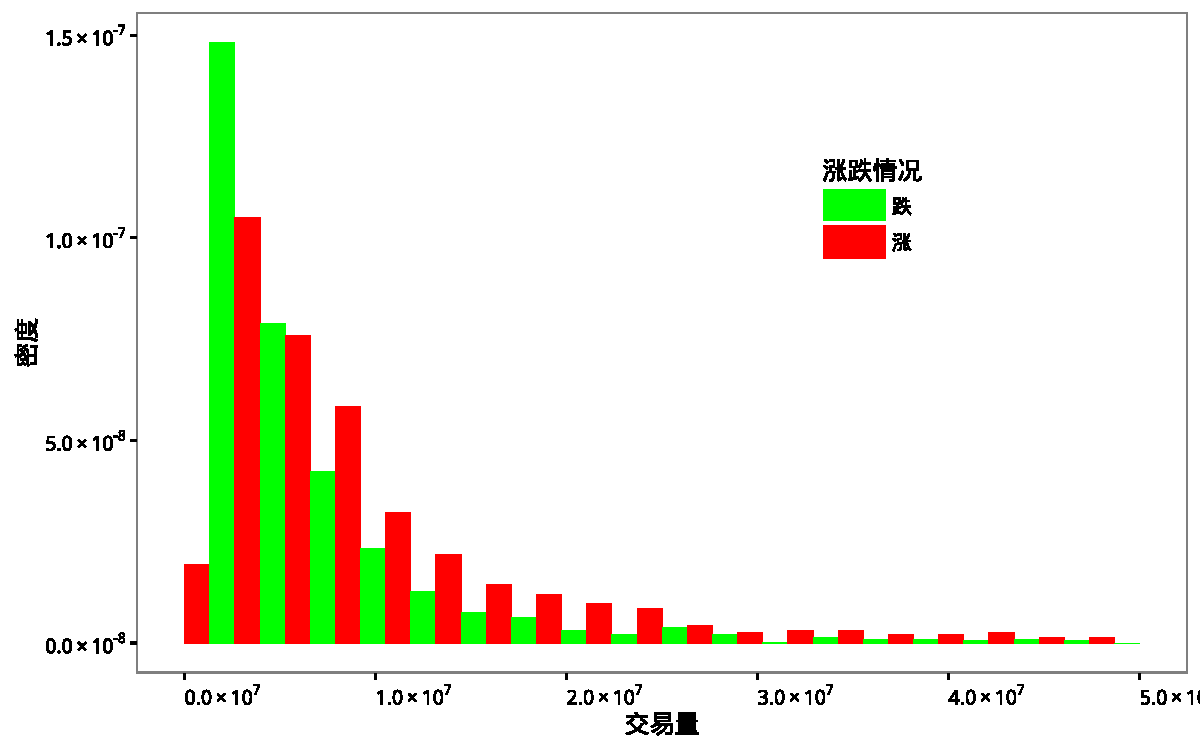
\includegraphics[width=150pt]{直方图1.pdf}
\includegraphics[width=150pt,height=110pt]{Rplot.png}
\caption{直方图和qq图}
\end{figure}
明显不满足正态分布的基本假设。
\end{frame}

\begin{frame}
\frametitle{Box-Cox变换}
对于不满足正态性假设的情况,一般有两种解决措施:
\begin{itemize}
\item 1.采取非参数检验的方式替代方差分析;
\item 2.采取适当的方法对原始数据做变换,使得数据满足正态性假设;
\end{itemize}
$Box-Cox$变换是统计建模中常用的一种数据变换,用于连续的响应变量不满足正态分布的情况。变换之后,可以一定程度修正数据的正态性水平。$Box-Cox$变换的公式如下所示:
\[ f(y)=\left\{ \begin{array}{ll}
\frac{y^{\lambda}-1}{\lambda} & \mbox{if}\lambda \neq 0,\\
log(y) & \mbox{otherwise.} \end{array} \right. \]
在本文中,我们采取的办法是使用$Box-Cox$变换修正原始数据的正态性水平。
\end{frame}

\begin{frame}
如下所示,我们选定$\lambda$为-0.1.
\frametitle{Box-Cox变换}
\begin{figure}
\centering
\includegraphics[width=210pt]{boxcox变换.png}
\caption{Box-Cox变换}
\end{figure}
\end{frame}

\begin{frame}
\frametitle{正态性检验}
如下是2013年6月3日成交量经过$Box-Cox$变换后直方图和qq图。
\begin{figure}[H]
\centering
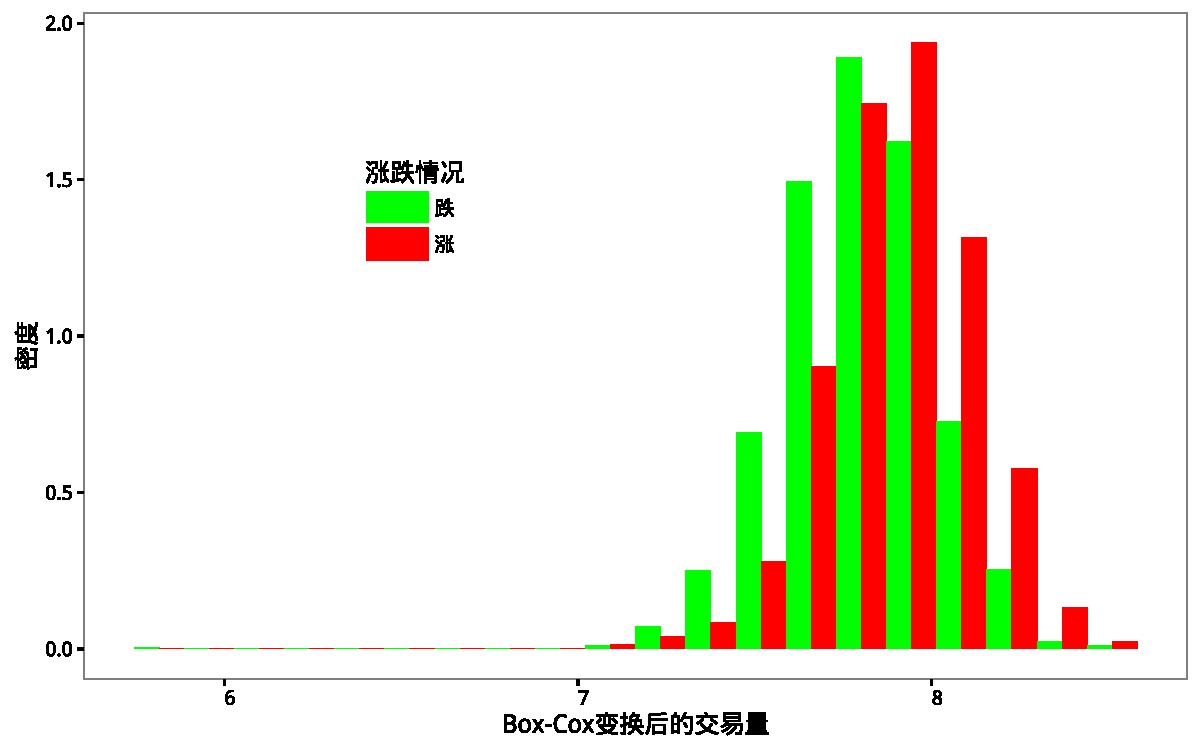
\includegraphics[width=150pt]{直方图2.pdf}
\includegraphics[width=150pt,height=110pt]{Rplot01.png}
\caption{直方图和qq图}
\end{figure}
我们可以认为数据已经满足了正态分布的基本假设。
\end{frame}

\begin{frame}
\frametitle{方差齐性检验}
我们计算了2016年6月3日,各水平下调整后的成交量的标准差,各水平的标准差如下:
\begin{table}[H]
\centering
\caption{方差齐性检验}
\begin{tabular}{cccccc}
\hline
	时间&状态&标准差&状态&标准差\\\hline
	2013-6-3&涨&0.21&跌&0.21\\
	\hline
\end{tabular}
\end{table}
如上表所示,各水平下的方差相差不大,我们认为数据满足了方差齐性检验。可以使用方差分析。
\end{frame}

\begin{frame}
\frametitle{方差分析}
$H_0:$一天之内上涨的股票和下跌的股票成交量相等; 

$H_1:$一天之内上涨的股票和下跌的股票成交量不相等。
\begin{table}[H]
\centering
\caption{方差分析}
\begin{tabular}{ccccccc}
\hline
	  时间   & & 自由度 & 平方和 & 均方 & F统计量 & p值 \\\hline
	2013-6-3& 组内 & 1 & 5.86 & 5.86 & 132.6 & $10^{-16}$ \\
          & 组间 & 2370 & 104.7 & 0.044 & &\\\hline
\end{tabular}
\end{table}
p值小于0.05,在95\%的显著性水平下认为这一天上涨股票和下跌股票的成交量不相等。
\end{frame}

\begin{frame}
\frametitle{扩展到九个横截面}
如下是各水平下的A股成交量的直方图、偏度系数与峰度系数。
\begin{figure}
\centering
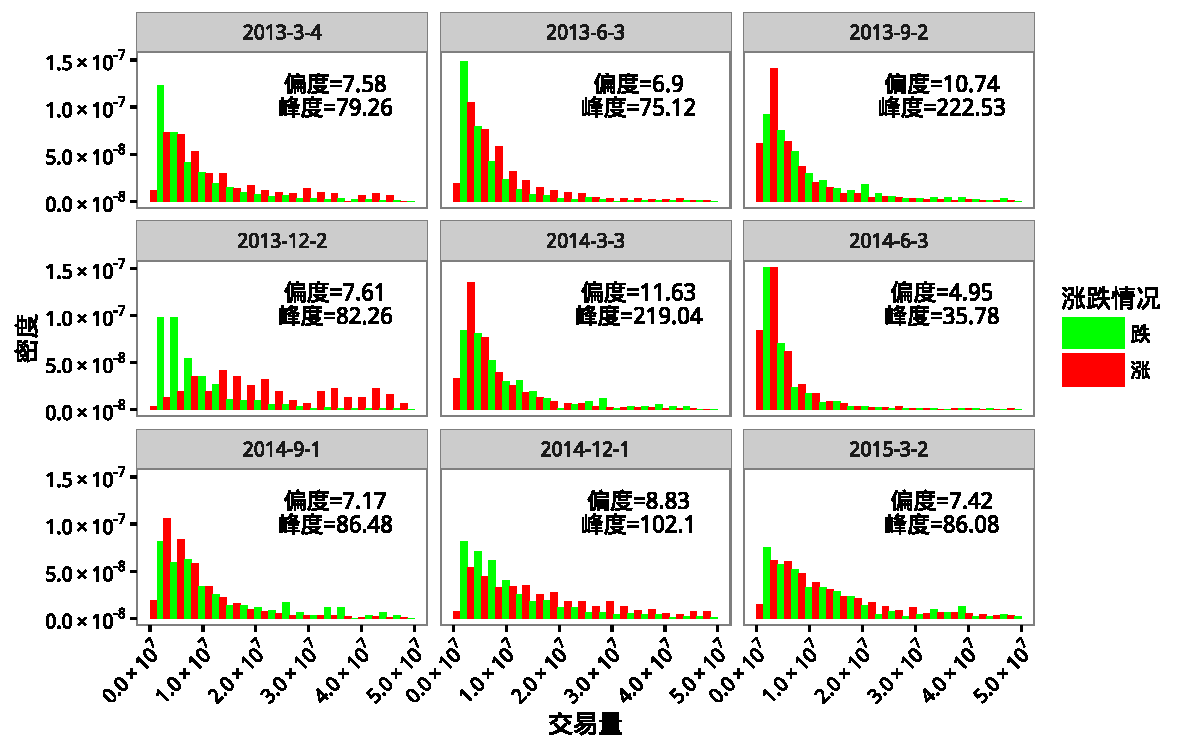
\includegraphics[width=270pt]{成交量直方图.pdf}
\caption{成交量直方图}
\end{figure}
\end{frame}

\begin{frame}
\frametitle{扩展到九个横截面}
如下是各水平下的A股调整后成交量的直方图、偏度系数与峰度系数。
\begin{figure}
\centering
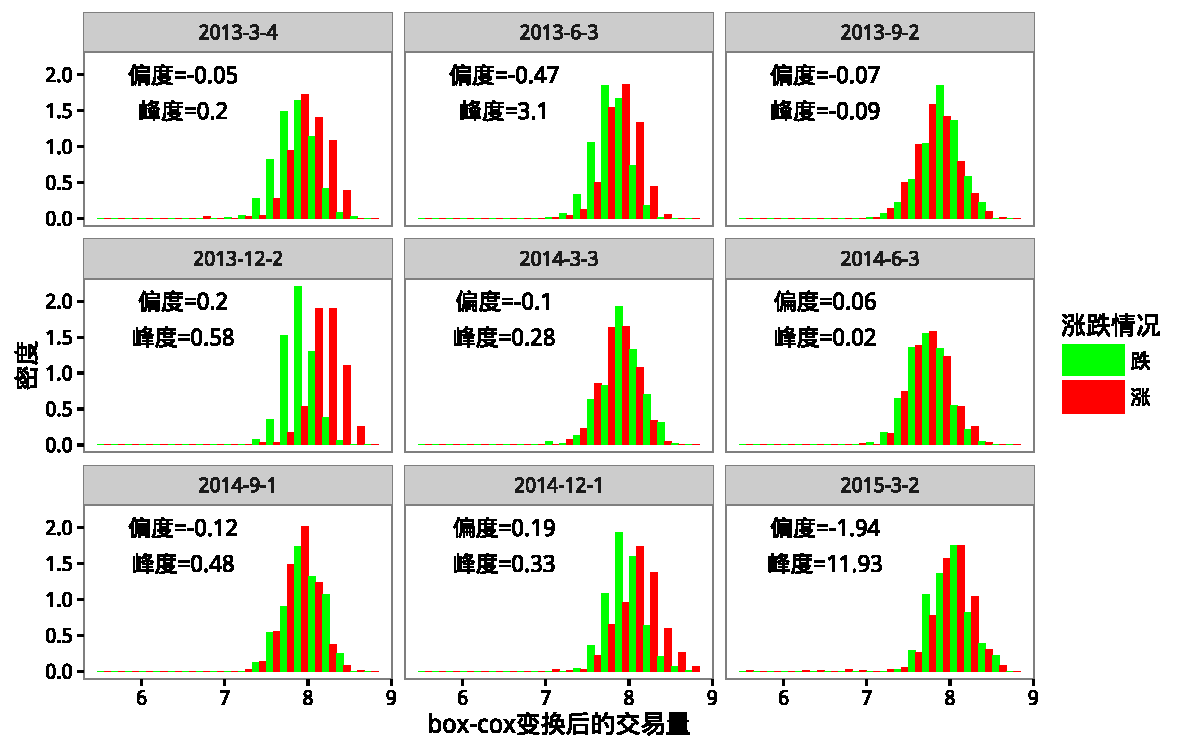
\includegraphics[width=270pt]{成交量直方图2.pdf}
\caption{成交量直方图}
\end{figure}
\end{frame}

\begin{frame}
\frametitle{扩展到九个横截面}
如下是各水平下的A股调整后成交量各水平下的方差:
\begin{table}
\centering
\caption{方差齐性检验}
\begin{tabular}{cccccc}
\hline
	时间&状态&标准差&状态&标准差\\\hline
	2013-3-4&涨&0.24&跌&0.23\\
	2013-6-3&涨&0.21&跌&0.21\\
	2013-9-2&涨&0.25&跌&0.24\\
	2013-12-2&涨&0.2&跌&0.18\\
	2014-3-3&涨&0.22&跌&0.24\\
	2014-6-3&涨&0.24&跌&0.24\\
	2014-9-1&涨&0.2&跌&0.22\\
	2014-12-1&涨&0.25&跌&0.21\\
	2015-3-2&涨&0.28&跌&0.24\\
	\hline
\end{tabular}
\end{table}
\end{frame}

\begin{frame}
\frametitle{扩展到九个横截面}
如下是各水平下的A股调整后成交量的方差分析结果:
\begin{table}[H]
\centering
\caption{方差分析}
\begin{tabular}{ccccccc}
\hline
	  时间   & & 自由度 & 平方和 & 均方 & F & p \\\hline
	2013-3-4& 组内 & 1 & 4.03 & 4.03 & 76.42 & $10^{-16}$ \\
	        & 组件 & 2389 & 125.84 & 0.053 &  & \\\hline
	2013-6-3& 组内 & 1 & 5.86 & 5.86 & 132.6 & $10^{-16}$ \\
          & 组间 & 2370 & 104.7 & 0.044 & &\\\hline
	2013-9-2& 组内 &1 & 7.0 & 7.0 & 115.6 & $10^{-16}$\\
          & 组间 & 2352 & 77.75 & 0.033 & & \\\hline
	2013-12-2& 组内 & 1 & 12.88 & 12.88 & 386.7 & $10^{-16}$ \\
          & 组间 & 2335 & 77.75 & 0.033 & & \\\hline
\end{tabular}
\end{table}
\end{frame}

\begin{frame}
\frametitle{扩展到九个横截面}
\begin{table}[H]
\centering
\caption{方差分析}
\begin{tabular}{ccccccc}
\hline
	  时间   & & 自由度 & 平方和 & 均方 & F & p \\\hline
2014-3-3& 组内 &1 & 1.93 & 1.93 & 38.65 & $5 \times 10^{-10}$\\
	        & 组间 & 2374 & 118.33 & 0.0498 & & \\\hline
	2014-6-3& 组内 & 1 & 0 & 0 & 0.072 & 0.789\\
	        & 组间 & 2304 & 130.5 & 0.0566 & & \\\hline
	2014-9-1& 组内 &1 & 0.82 & 0.82 & 19.81 & $9\times 10^{-6}$\\
	        & 组间 & 2302 & 95.01 & 0.0413 & & \\\hline
	2014-12-1& 组内 & 1 & 7.54 & 7.54 & 149.7 & $10^{-16}$\\
	         & 组间 & 2289 & 115.31 & 0.05 & & \\\hline
	2015-3-2& 组内 & 1 & 0.11 & 0.11 & 1.466 & 0.226\\
	        & 组间 & 2373 & 176.35 & 0.074 & & \\\hline
\end{tabular}
\end{table}
\end{frame}

\begin{frame}
\frametitle{结论}
在大部分的分组中,方差分析检验的结果都拒绝原假设,认为上涨和下跌的股票成交量有显著性差别,但是在2014年6月3日和2015年3月16日,方差分析不能拒绝原假设,在这两天,没有足够的理由认为上涨股票和下跌股票的成交量存在显著性差别。
\end{frame}

\end{document}